\chapter{Alternative schemes for computing extracellular potentials from neural activity}
\label{sec:Schemes}

The extracellular potentials that we have analyzed so far have been computed using the two-step Hodgkin-Huxley-Cable + Volume Conductor (HHC+VC) scheme (Fig. \ref{Schemes:fig:schemes}A), which is based on the theory that we presented in Chapters \ref{sec:Neuron}-\ref{sec:Sigma}. 

The HHC+VC scheme has two main limitations. Firstly, it does not account for so-called \textit{ephaptic effects} of extracellular variables (computed in step 2) on the neurodynamics (computed in Step 1). Since in Step 1 computes the neurodynamics under the assumption that the extracellular potential is constant (zero), and in Step 2 uses this neurodynamics to compute a non-zero extracellular potential, it is not self-consistent. Secondly, the HHC+VC scheme does not account for any effects that varying ion concentrations may have on the neurodynamics or on the extracellular potential, but implicitly assumes that all ion concentrations remain constant under the simulated period. 

In this chapter, we briefly summarize some alternative schemes (Fig. \ref{Schemes:fig:schemes}).
Among all existing schemes, HHC+VC is the by far most "user-friendly" scheme, and is thought to be sufficient for most purposes. However, for purposes where it is not, one should consider using one of the alternative schemes, which account ion concentration effects on the extracellular potential (Fig. \ref{Schemes:fig:schemes}B), ephaptic feedback from extracellular dynamics on neurodynamics (Fig. \ref{Schemes:fig:schemes}C) or both (Fig. \ref{Schemes:fig:schemes}D).


\begin{figure}[!ht]
\begin{center}
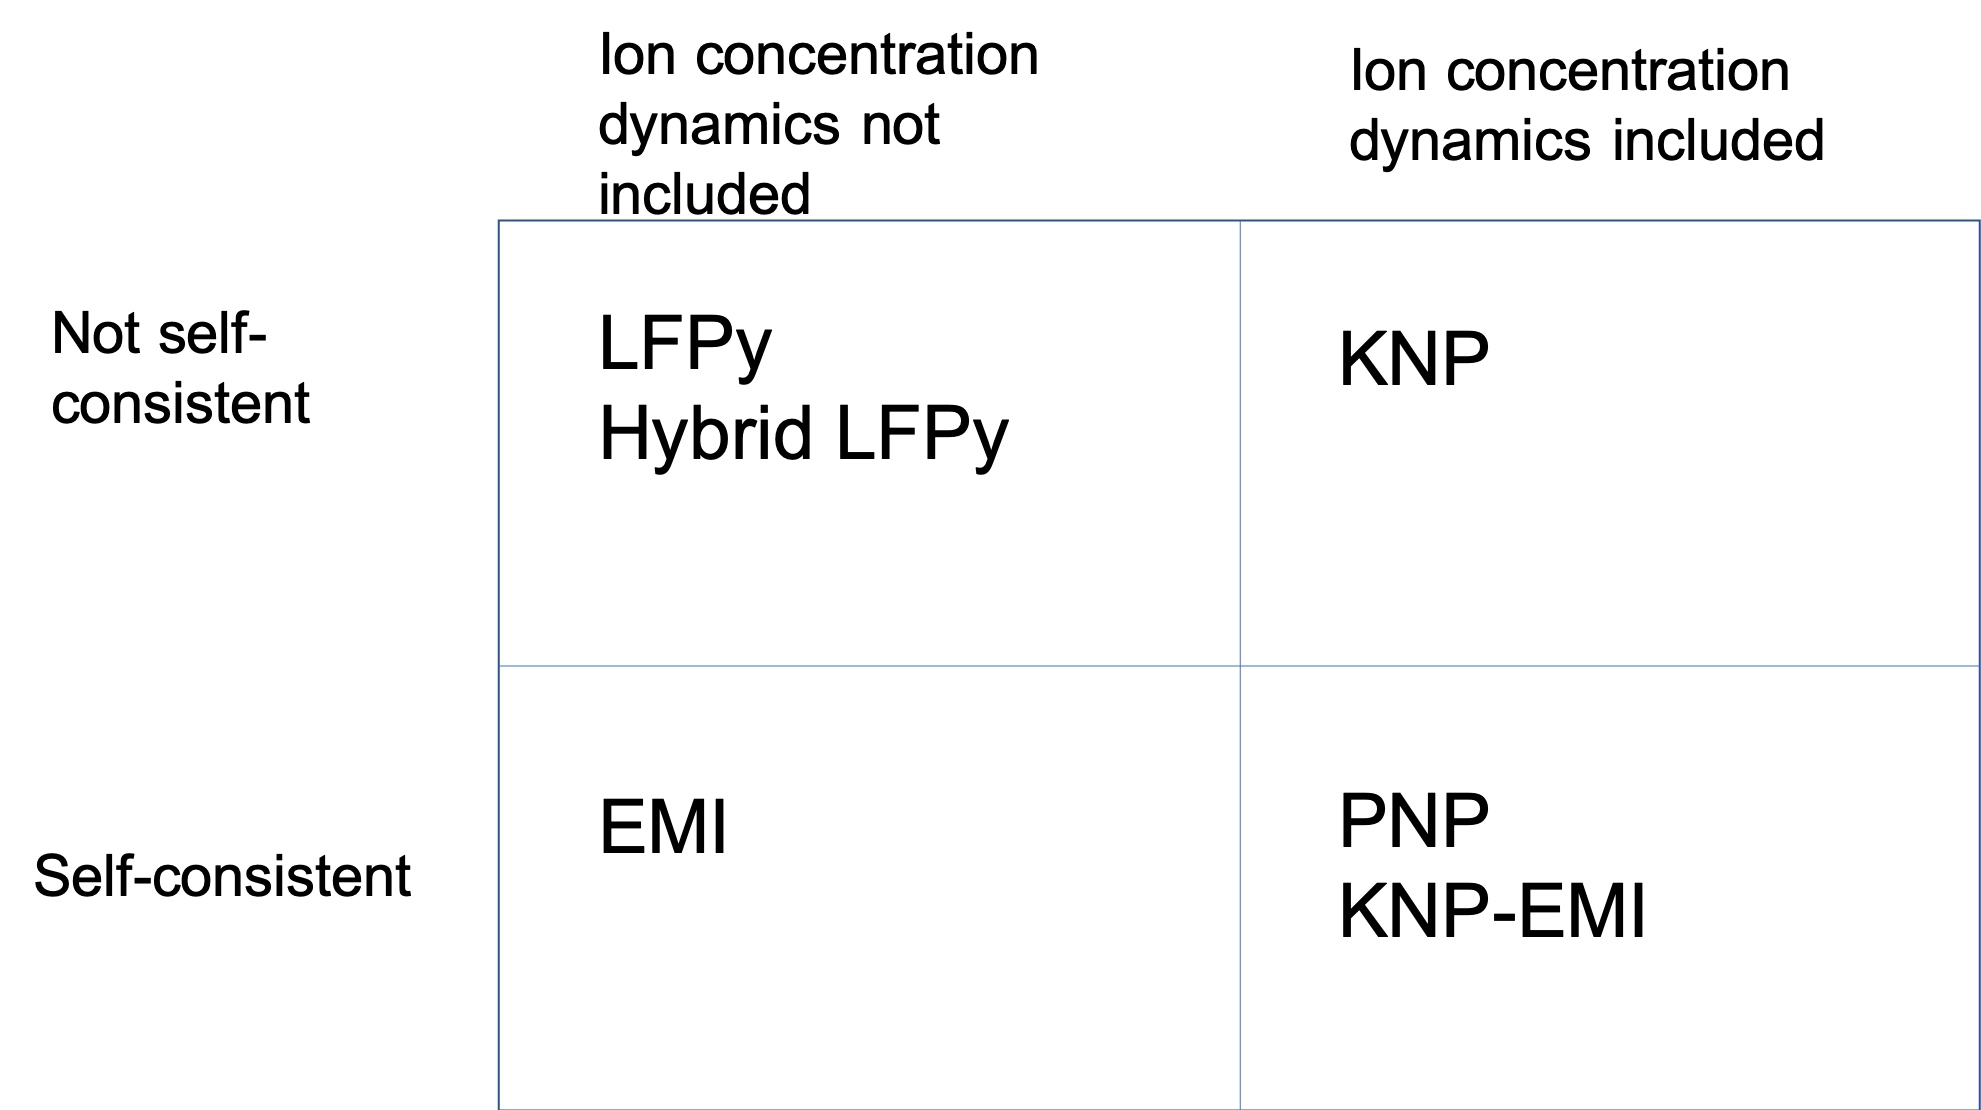
\includegraphics[width=0.8\textwidth]{Figures/Schemes/Schemes.png}
\end{center}
\caption{\textbf{Overview of schemes for computing extracellular dynamics.} The extracellular potential largely originates from neuronal transmembrane currents, illustrated for a simple (two-compartment) neuron, with currents that cross its membrane in the form of a current sink $I_1$ in one compartment, and a current source $I_2$ in the other (green arrows). {\textbf (A)}: HHC+VC: Two-step procedure which (Step 1) computes transmembrane neural currents in an independent simulation using Hodgkin-Huxlley-Cable (HHC) formalism, and then (Step 2) from these computes the extracellular potential using Volume Conductor (VC) theory. {\textbf (B)}: HHC + ED: Two-step scheme, which (Step 1) computes currents and ion fluxes in an independent simulations based on HHC, and (Step 2) from these computes the changes in the extracellular potential and ion concentrations using an electrodiffusive (ED) framework. {\textbf (C)}: VC + VC: Computes intracellular and extracellular electrodynamics simultaneously on a unified VC framework. Accounts for ephaptic effects, but assumes ion concentrations to be constant. {\textbf (D)}: ED + ED: Computes intracellular and extracellular ion concentration- and electrodynamics simultaneously on a unified electrodiffusive framework based on the Nernst-Planck equation. Account for ephaptic effects and ion-concentration dynamics. 
}
\label{Schemes:fig:schemes}
\end{figure}


%%%%%%%%%%%%%%%%%%

\section{\blue{Self-consistent electrodiffusive schemes}}
\label{sec:Schemes:complete}
\index{Electrodiffusion} \index{Nernst-Planck equation}


When modeling an electrodiffusive process, we keep track of the ion concentration dynamics of each individual ion species. The fundamental equation for doing that is the Nernst-Planck equation for the flux density (${\bf j_k}$ of an ion species $k$:
\begin{equation}
{\bf j_k} = - D_k {\bf \nabla} c_{k} - \frac{D_k z_k c_k}{\psi} {\bf \nabla} \phi, 
\label{Schemes:eq:JNP}
\end{equation}
where ${D}_k$ is the diffusion constant (units $\mathrm{m^2/s}$), $z_{k}$ is the valency of ion species $k$, and $\psi=RT/F$ (units V) is defined by the gas constant ($R$), Faraday's constant ($F$) and the temperature ($T$). The first term on the right is Fick's law for diffusion, while the second term accounts for ions migrating in the electric field.  In eq. \ref{Schemes:eq:JNP}, the the electrical mobility of the ions is $D_k/\psi$, and thus linearly related to their diffusion constant. This relationship is called the Einstein relation\index{Einstein relation}, and is valid for dilute solutions such as the extracellular fluid \cite**{Grodzinsky2011}.

If we combine eq. \ref{Schemes:eq:JNP} with the requirement of ion conservation:
\begin{equation}
\frac{\partial c_k}{\partial t} = -\nabla \cdot {\bf j_k},
\label{Schemes:eq:general_ionconservation}
\end{equation}
we get the Nernst-Planck continuity equation:
\begin{equation}
\frac{\partial c_k}{\partial t} = {\bf \nabla} \cdot \left[{D_k} {\bf \nabla} c_k + \frac{D_k z_k c_k}{\psi}{\bf \nabla} \phi \right].
\label{Schemes:eq:NP}
\end{equation}

In principle, we can compute all ionic concentrations and their coupling to the electrical potential by requesting that eq. \ref{Schemes:eq:NP} should be fulfilled at all points in space, including both the extracellular space, the intracellular space and the membranes separating them. Eq. \ref{Schemes:eq:NP} then gives us one equation for each individual ion concentration $c_k$, and to solve the system of equations, we are in need an additional equation for the additional variable $\phi$, the electrical potential which couples the dynamics of the individual ion species. There are two main approaches to this, the so-called \textit{Poisson-Nernst-Planck (PNP)} framework, or the so-called \textit{electroneutral} framework, both of which we will introduce below. 


\subsection{\blue{What is a diffusion potential?}}
\label{sec:Schemes:LJpot}
\index{Diffusion potential}
Before we start introducing electrodiffusive schemes, we may establish an intuitive understanding of the link between ion concentration dynamics and electric potentials by considering a simple two-compartment system with two ionic solutions interacting at a junction  (Fig. \ref{Schemes:fig:diffpot}). Let us assume that the left compartment contains a high-concentration solution of NaCl, while the right compartment contains a low-concentration solution of NaCl (Fig. \ref{Schemes:fig:diffpot}A). Let us also assume that initially, both compartments are perfectly electroneutral, i.e.,the amounts of Na$^+$ and Cl$^-$ within each compartment are equal. No  electrical forces will then be present, and the initial system dynamics will be driven exclusively by diffusion. 

\begin{figure}[!ht]
\begin{center}
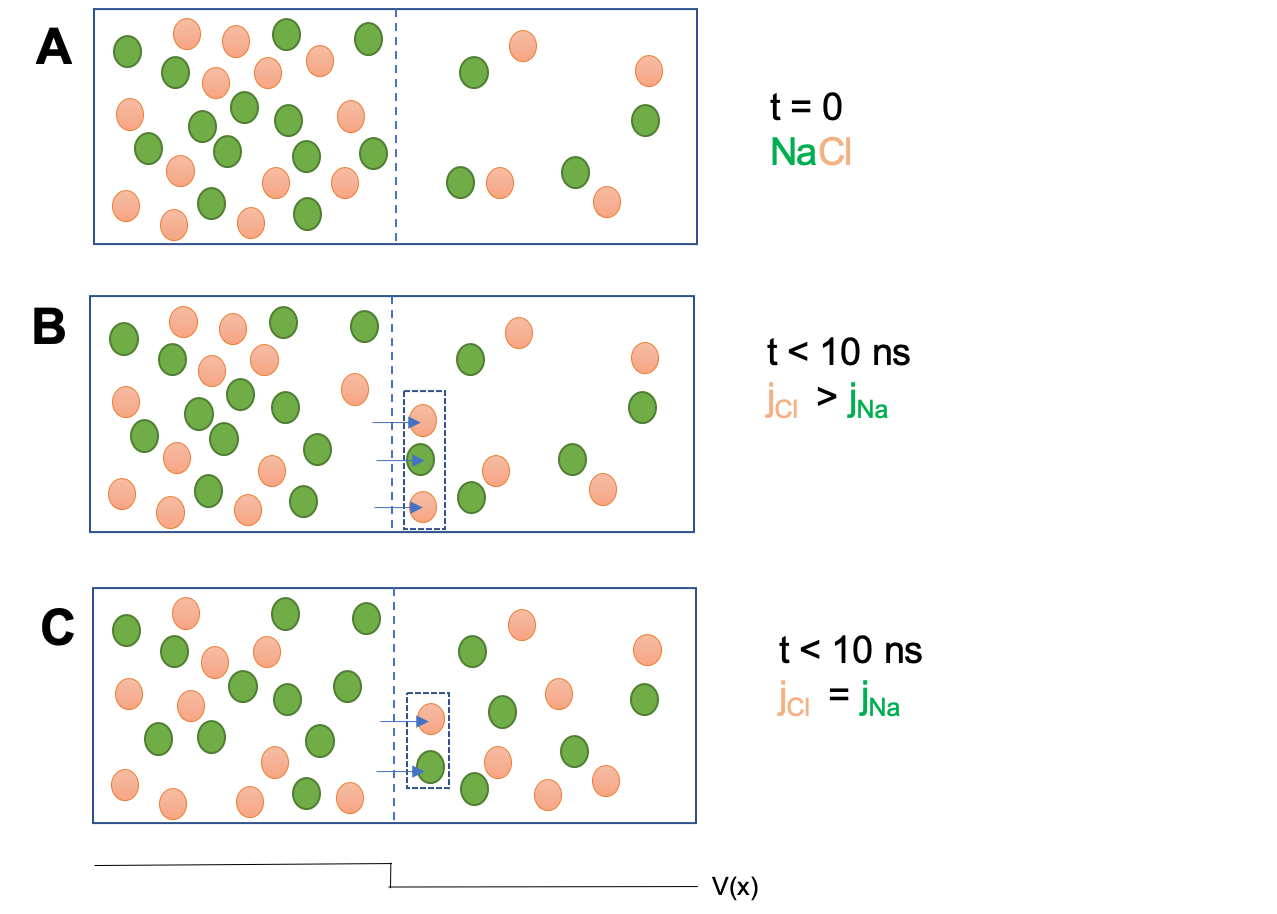
\includegraphics[width=0.8\textwidth]{Figures/Schemes/Diffusionpot.png}
\end{center}
\caption{\textbf{Diffusion potential at the junction between two ionic solutions}. ({\bf A}) Initial condition with high concentration NaCl in the left compartment and low concentration NaCl in the right compartment. ({\bf B}) Since $D_{Cl} > D_{Na}$, we initially expect the flux of Cl$^-$ to be higher than the flux of Na$^+$. ({\bf C}) The net charge transfer in ({\bf B}) will give rise to a potential difference $\phi_d$ between the two compartments, which will prevent further charge accumulation. }
\label{Schemes:fig:diffpot}
\end{figure}

Without solving any equations, we realize both Na$^+$ and Cl$^-$ will diffuse towards the low-concentration compartment on the right-hand-side. The diffusion speed for the various ions will be proportional to their respective diffusion constants, and from Table \ref{Sigma:tab:diffconsts}, we know that $D_{Na} = 1.33 \times 10^{-9}$ m$^2$/s, and $D_{Cl} = 2.03 \times 10^{-9}$ m$^2$/s in dilute solutions. Since $D_{Cl} > D_{Na}$, the rightward diffusive flux of Cl$^-$ will initially be larger than that for Na$^+$  (Fig. \ref{Schemes:fig:diffpot}B). Diffusion thus acts as a charge separation process, causing an excess of positive charge in the left compartment and negative charge in the right compartment. Because of this, a potential difference ($\Delta \phi_d$) will arise between the compartments. Since $\Delta \phi_d$ stems from a diffusion process, it is often called the \textit{diffusion potential} \index{Diffusion potential}. 

The diffusion potential will oppose the on-going charge separation process by causing an electrical push on the anions (Cl$^-$) in the leftward direction, reducing the net rightward flux of Cl$^-$. Similarly, it causes a rightward pull on the cations (Na$^+$), increasing the net rightward flux of Na$^+$. When it is gets big enough, $\Delta \phi_d$ will stabilize the system in a so-called quasi-steady state, where the net fluxes of Na$^+$ and Cl$^-$ have the same magnitude, and no further charge separation will take place (Fig. \ref{Eldiff:fig:diffpot}C). It has been shown that, in the extracellular medium of the brain, it only takes in the order of 10 ns to reach this quasi-steady state \cite**{Solbra2018}. Note that in the quasi-steady state, $\Delta \phi_d$ will still vary with time (hence the term "quasi"), and eventually become zero when the system is equilibrated and the ion concentrations are the same in the two compartments. However, whereas the quasi-steady state is reached within a few nanoseconds, the concentration-equilibration process occurs at an entirely different time scale and normally takes seconds to minutes.

Since it happens so fast, computer simulations of the charge separation process must be run with a sub-nanosecond time resolution. To simulate it is therefore computationally demanding, and not even feasible for large systems. Fortunately, one can for many purposes obtain accurate predictions of both $\Delta \phi_d$ and ion concentration dynamics by using an electroneutral mathematical framework that does not model the charge relaxation process explicitly, but instead derives an analytical expression for the quasi-steady state potential, and assumes that the system is always in quasi-steady state. We shall introduce the modeling frameworks for electrodiffusive processes in the following sections. 

Note that the diffusion potential arises due to differences in diffusion constants between different ions present  (cf. Table \ref{Sigma:tab:diffconsts}). If all ions had identical diffusion constants, there would be no charge separation and thus no diffusion potential. 

Note also that the reversal potential of an ion channel (eq. \ref{Neuron:eq:revpots}) is essentially a single-ion diffusion potential, and the leakage reversal potential (eq. \ref{Neuron:eq:Eleak_GHK}) is a diffusion potential depending on the differences in passive membrane permeabilities (playing the role of diffusion constants) of the various ion species.

In electrolyte theory, the diffusion potential is often called the \textit{liquid-junction potential} \index{Liquid-junction potential}, since it is most pronounced at the junction between two different ionic solutions \cite**{Sokalski2001}. Liquid-junction potentials are a common problem when recording neural membrane potentials using patch clamp experiments. Through a process similar to that depicted in Fig. \ref{Schemes:fig:diffpot}, only involving a larger number of different ion species, 
the liquid-junction potentials develop at the junction between the pipette solution and the extracellular (or bath) solution, and give rise to a constant offset in the recordings, which must be estimated and corrected for \cite**{barry1991}. Their magnitude depend on the composition of the various ion solutions, but are typically on the order of a few millivolts. 

Whereas the Nernst-Potential and the liquid-junction potentials in patch clamp experiments are somewhat familiar examples of diffusion potentials in neuroscience, diffusion potentials in the bulk solutions or the intra- or extracellular space tend to be smaller in magnitude, and have not been that much studied in neuroscience. Below, we will outline the physical theory for determining the electric potential in electrodiffusive processes.


\subsection{\blue{The Poisson-Nernst-Planck (PNP) framework}}
\label{sec:Schemes:PNP}
\index{Poisson-Nernst-Planck equations}
The physically most detailed approach for defining $\phi$ in eq. \ref{Schemes:eq:NP}) is to use Poisson's equation from electrostatics:
\begin{equation}
\nabla^2 \phi = -\rho/\epsilon
\label{Schemes:eq:poisson}
\end{equation}
Here $\epsilon$ is the (local) permittivity of the medium, and in the last step, we have expressed the local charge density $\rho$ as a function of the ionic concentrations. 
\begin{equation}
\rho = F\sum_k z_k c_k + \rho_0.
\label{Schemes:eq:PNPrho}
\end{equation}
When we model ion concentrations, we normally do not include absolutely all ion species that are present, but rather chose to keep track of the most important ones (such as Na$^+$, K$^+$, Cl$^-$ and Ca$^{2+}$). A static charge density $\rho_0$\index{Static charge density} was therefore added to eq.\ref{Schemes:eq:PNPrho} to account for all charges not included in the set $c_k$. 

The PNP equations (eq. \ref{Eldiff:eq:NP} together with eq. \ref{Schemes:eq:poisson}) can in principle be solved for arbitrary complex geometries using numerical methods, like the Finite Element Method (FEM). 

To apply the PNP scheme within a neuroscience context poses several challenges. Firstly, one needs to represent the geometry and properties of the cellular membranes. In principle, this could be achieved through having spatially and temporally varying diffusion coefficients $D_k$. However, the resolution with which one needed to represent $D_k$ would then be extremely high. Whereas $D_k$ could have a constant value in the intra- and extracellular bulk solutions, $D_k$ would over the membranes be (i) different in different spatial directions (i.e., normal to membrane surface versus parallel to membrane surface), (ii) vary with the very fine spatial resolution of an ion channel, and (iii) also be time dependent due to the opening/closing of ion channels. Unless the PNP scheme is applied to specifically model currents inside ion channels on a very small spatial scale (see e.g., \cite**{Gardner2011, Zheng2011}), such a fine-grained tensor description of $D_k$ does not seem like a reasonable approach. 

Instead, it is common to rather have the PNP equations being defined in two disjoint domains - the intra and extracellular - and to couple the dynamics in these two domains by introducing suitable boundary conditions at the membrane. In many applications, the membrane dynamics is then based on a Hodgkin-Huxley (HH) type formalism (c.f., Section \ref{sec:Neuron:membranecurrents}) also in PNP type modeling (see e.g., \cite**{Lopreore2008, Pods2013, Gardner2015, Pods2017}). When applying a HH formalism in this context, all transmembrane currents are made ion specific, i.e., they are described in terms of ionic fluxes over the membrane, so that for example a Na$^+$ current density ($i_{Na}$) in the standard HH formalism would need to be replaced with a Na$^+$ flux density, $j_{Na} = i_{Na}/(Fz_k)$. The leakage current ($i_L$ in eq. \ref{Neuron:eq:HHleak}) is in standard HH applications non-specific in terms of which ions that mediate it, but will in a PNP context have to be made ion specific by decomposing it into specific leakage fluxes of the various ions that are involved (see e.g., \cite**{Pods2013}). Apart from that, the HH formalism for membrane mechanisms can be applied in its original form also in an electrodiffusive context.

A second challenge with the PNP system of equations is that solving them is extremely computationally demanding. One reason for this is that the concentrations of ions in a finite volume of space are almost so that the net positive and negative charges outbalance, meaning that the medium is very close to electroneutral. A non-zero charge density ($\rho$) thus reflects a deviance from electronutrality, and it has been estimated that this deviance typically involves only a fraction $\sim 10^{-9}$ of the ions present \cite**{Aguilella1987}. An accurate prediction of $\rho$ from eq. \ref{Schemes:eq:PNPrho} thus requires an extreme precision in the modeling of the ionic concentrations $c_k$. Another, related, reason is that the charge-relaxation time in the extracellular solution, i.e., the time scale that $\rho$ varies on, is in the order of nanoseconds. In addition, any non-zero charge density in neural tissue is predominantly resolved in nano-meter thick layers around neuronal membranes \cite**{Grodzinsky2011, Gratiy2017}. Simulations of $\rho$ therefore require a spatiotemporal resolution smaller than nanometers and nanoseconds, and thus a very fine-grained description of the tissue where neuronal, glial and extracellular geometries are explicitly defined.

Due to its computational demand, the PNP framework is not suitable for estimating dynamics at the level of tissue, and the framework does not lend itself to be coarse-grained. Applications in neuroscience have therefore been limited to studies of electrodiffusive processes taking place on a very tiny spatiotemporal scale, such as in dendritic spines or near and inside membranes (see e.g., \cite**{Leonetti2004, Lu2007, Lopreore2008, Nanninga2008, Gardner2011, Zheng2011, Pods2013, Gardner2015, lagache2019, cartailler2019}). See \cite**{Savtchenko2017} for a review of applications in neuroscience.


\subsection{\blue{The electroneutral framework}}
\label{sec:Schemes:electroneutral}
\index{Electroneutral}
An alternative to the PNP framework is to replace the Poisson equation (eq. \ref{Schemes:eq:poisson}) with the approximation that the bulk solution is electroneutral:
\begin{equation}
F \sum_k z_k c_k + \rho_0 = 0.
\label{Schemes:eq:electroneutral}
\end{equation}
In practice, it is often more convenient to impose the electroneutrality approximation on differential form:
\begin{equation}
F \sum_k{z_k \frac{\partial c_k}{\partial t}} = 0.
\label{Schemes:eq:electroneutral2}
\end{equation}

The electroneutrality approximation (eq. \ref{Schemes:eq:electroneutral} or \ref{Schemes:eq:electroneutral2}) can be imposed as a constraint when solving eq.\ref{Schemes:eq:NP} by use of some numerical method. The constraint determines what $\phi$ must be at all points in space for there to be no charge accumulation anywhere in the extracellular or intracellular bulk solutions, which, as soon as reference point ($\phi = 0$) is set, has a unique solution.

To explain how the electroneutral framework differs from the PNP framework, we may use our previous cartoon example (Fig. \ref{Schemes:fig:diffpot}) as a reference. While the PNP framework explicitly models the nanosecond-fast charge relaxation process (Fig. \ref{Schemes:fig:diffpot}B), the electroneutral framework circumvents it by assuming (and ensuring) that the system is always in quasi-steady (Fig. \ref{Schemes:fig:diffpot}C). It has been shown that this is a good approximation on spatiotemporal scales larger than micrometers and microseconds \cite**{Grodzinsky2011, Pods2017, Solbra2018}. The advantage with this approach is that it, unlike PNP, gives stable solutions with an arbitrary coarse spatiotemporal resolution.

We note that the electroneutrality constraint (eq. \ref{Schemes:eq:electroneutral} or \ref{Schemes:eq:electroneutral2}) only applies to the intra- and extracellular bulk solutions, so that the membrane dynamics must be dealt with separately. Firstly, one must then define the equations that govern the membrane dynamics. A natural choice for this is, again, to use an ion-specific HH-like formalism \cite**{Mori2006, Mori2009, Pods2017, ellingsrud2020}. 

Secondly, the electroneutrality condition does not apply at the membrane, where a non-zero membrane (surface) charge density ($\eta^{mem}$ (C/m$^2$)) builds up the membrane potential according to the capacitor relationship:
\begin{equation}
c_m \phi_{m} = \pm \eta_{r}^{mem},
\label{Schemes:eq:rhocap}
\end{equation}
or its temporal derivative: 
\begin{equation}
i_{cap} = \pm \frac{\partial \eta_{r}^{mem}}{\partial t},
\label{Schemes:eq:rhocapt}
\end{equation}
Here, $c_m$ (F/m$^2$) in eq. \ref{Schemes:eq:rhocap} is the specific membrane capacitance, and the left hand side of eq. \ref{Schemes:eq:rhocapt} follows the definition is the capacitive membrane current density $i_{cap}$  (eq. \ref{Neuron:eq:HHcap}). In both equations, $r$ takes the indices $i$ (intracellular side of the membrane) or $e$ (extracellular side of the membrane), and the plus-sign should be used for $r=i$, and the minus-sign for $r=e$, a convention that follows from the definition $\phi_{m} = \phi_{i} - \phi_{e}$. The intra- and extracellular membrane charge densities in eq. \ref{Schemes:eq:rhocap} or their derivatives in \ref{Schemes:eq:rhocapt} are equal in magnitude and opposite in sign, since the charge stored on one side of a capacitor always balances the charge stored on the other side. 

For the electroneutrality constraint at the membrane (eq. \ref{Schemes:eq:rhocap} or \ref{Schemes:eq:rhocapt}) to be useful, $\eta_{r}^{mem}$ must be expressed in terms of the ion concentrations. That is, one needs an additional condition to specify the composition of ions that constitute $\eta_{r}^{mem}$ in eq. \ref{Schemes:eq:rhocap} or mediate $i_{cap}$ in eq. \ref{Schemes:eq:rhocapt}, so that ion conservation and a consistent charge-concentration relationship  at all points in space is ensured. Previous schemes for implementing the electroneutral framework vary somewhat in the approach taken to this:

\begin{itemize}
\item The electroneutral scheme with internal boundary conditions at membranes (ENM), derived the concentration profile of the membrane charge density $\eta_{r}^{mem}$ from a set of constraints as to how ion concentrations are distributed within the Debye-layer \cite**{Mori2006, Mori2009, Pods2017}.

\item The Kirchhoff-Nernst-Planck (KNP) scheme did not resolve Debye-layer concentrations, but let the membrane concentration profile follow from an assumption regarding how much various ion species contributed to the capacitive membrane current $i_{cap}$ \cite**{ellingsrud2020}.
\end{itemize}

Both electroneutral schemes (ENM and KNP) were designed so that the membrane concentration profiles were functions of, and similar to, the concentration profiles in the bulk solution close to the membrane. Although they differ in implementation details, the two schemes should be close to equivalent from a physics point of view, except at Debye layer-resolution close to the membrane.  In practice, only a very tiny fraction of the ions present are involved in building up the membrane potential, and the choice as to which ion species that actually constitute the membrane charge in eq. \ref{Schemes:eq:rhocap} or \ref{Schemes:eq:rhocapt} is probably quite unimportant for the overall system dynamics.

Like the PNP scheme, both versions of the electroneutral scheme must be solved on some numerical framework. While the electroneutral frameworks are computationally much more efficient than the PNP framework, they are still too heavy to allow for simulations of large systems of neurons described with explicit geometries on today's computers. To our knowledge, the largest system that so far has been simulated in 3D on an electroneutral framework is small piece of tissue containing a bundle of 9 axons described with idealized geometries \cite**{ellingsrud2020}.


\subsection{\blue{Domain models}}
\label{sec:Schemes:domain}
\index{Domain models}
A different category of electroneutral models have been inspired from by the bi-domain model by Eisenberg \cite**{eisenberg1970}, which has previously been used to simulate cardiac tissue \cite**{henriquez1993, sundnes2006, Mori2008}. 

In this category, the most advanced models for brain tissue are the tri-domain models, where three the domains represent (i) neurons, (ii) extracellular space, and (iii) a glial syncytium, i.e., a populations of gap-junction coupled glial cells \cite**{OConnell2016, tuttle2019}. Simpler, related models include the bi-domain model for neurons and extracellular space \cite**{Mori2015}, or 1D models of glial K$^+$ buffering, where only the glial and extracellular domain were included \cite**{Gardner-Medwin1983, Chen2000, Halnes2013}.

The domain models do not model individual cells, but represents tissue as a (volume-averaged) continuum. All domains "exist" in parallel at each point in space, and are defined through a set of domain-specific variables (e.g., domain-voltage, domain-ion concentrations, domain-osmolarity, domain-volume fractions etc.). The domains interact locally through a set of (Hodgkin-Huxley type) membrane mechanisms, while spatial electrodiffusive transports may occur \textit{within} the domains. 

In the tri-domain models \cite**{OConnell2016, tuttle2019}, intra-domain ion transport was assumed to occur in the glial and extracellular domain, but not the neural domain. The rationale behind that assumption was that a type of glial cells called astrocytes tend to be gap-junction coupled into a syncytium. In the syncytium, the intracellular space is more or less continuous in the same way that the extracellular space is continuous. Transport processes within the syncytium is then equivalent to extracellular transport in the sense that both take place in a continuous, tortous space. In contrast, neurons do not form synciti, and are "local" in the sense that no intracellular transport over distances occur within the neural domain (Fig.\ref{Schemes:fig:domainmodel}). 

\begin{figure}[!ht]
\begin{center}
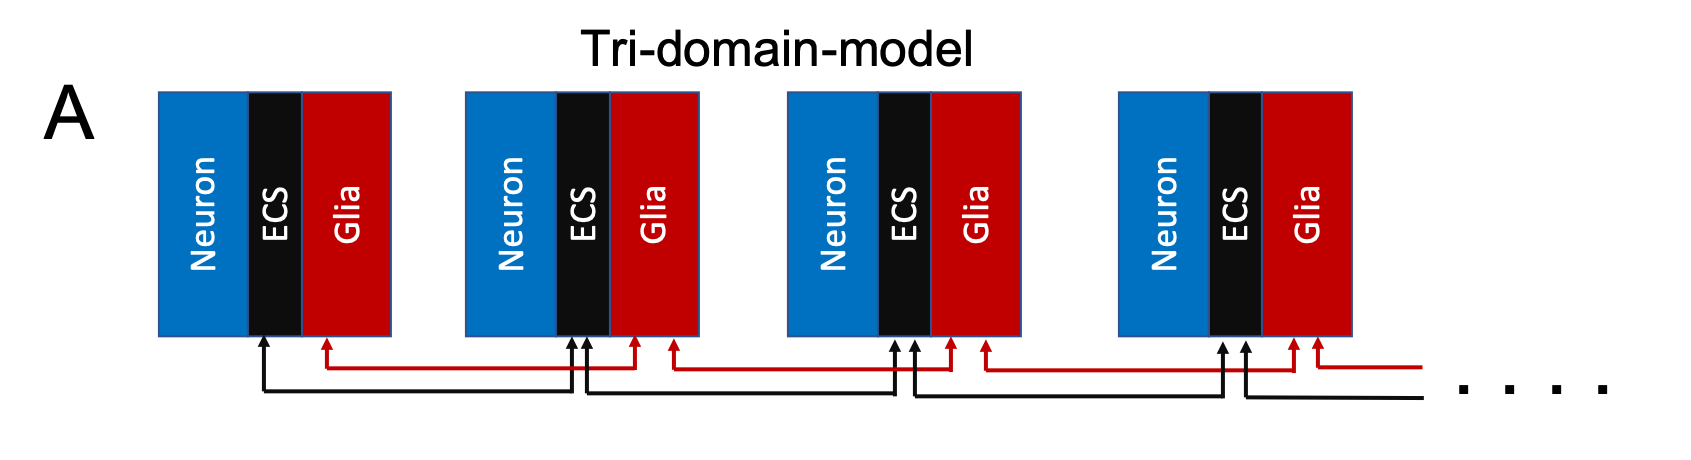
\includegraphics[width=0.8\textwidth]{Figures/Schemes/Tridomain.png}
\end{center}
\caption{\textbf{Tri-domain model of brain tissue.} The domains represent neurons, extracellular space (ECS) and glial cells. The domains interact locally through transmembrane currents. Spatial ellectrodiffusion (arrows) occur within the ECS and glia domains, but not in within neuronal domain.The spatial dynamics can, in principle, occur in all directions (3D),but a 1D illustration was used in the figure. 
}
\label{Schemes:fig:domainmodel}
\end{figure}

Domain models are suited to model brain dynamics taking place on large spatiotemporal scale, such as the wave of K$^+$ and the slow, DC-like diffusion potentials and glial buffering potentials that take place during the pathology of spreading depression \cite**{Mori2015, OConnell2016, tuttle2019}. As these models treat brain tissue as a homogeneous, coarse-grained continuum, they are not suited to model the faster fluctuations of extracellular potentials which are recorded in MUA, LFP and EEG, as these depend strongly on morphologies of neurons \cite**{Einevoll2013}. 


%%%%%%%%%%%%%%%%%%%%%%%%%%%%

\section{\blue{Two-step scheme for extracellular electrodiffusion surrounding active neurons}}
\label{sec:Schemes:KNP}
In the two-step, Hodgkin-Huxley-Cable + Kirchhoff-Nernst-Planck (HHC+KNP), scheme, the neurodynamics is computed in an independent step (Step 1), and assumed to be unaffected by whatever goes on in the extracellular space. In the next step (Step 2), the neuronal transmembrane output is treated as an "external input" source to the extracellular medium \cite**{Halnes2016, Solbra2018}. 

The HHC+KNP scheme thus adopts the approach of the standard HHC+VC framework (Chapter \ref{sec:LFPy}), but with the volume conductor theory used in the latter replaced with the electroneutral electrodiffusive Kirchhoff-Nernst-Planck (KNP) framework \cite**{Halnes2016, Solbra2018, ellingsrud2020}. 

Compared to the self-consistent electrodiffusive schemes presented in Section \ref{sec:Schemes:complete}, the HHC+KNP scheme is less computationally demanding, and lends itself to be combined with HHC-simulations of morphologically detailed neuron models. However, like the HHC+VC scheme, the HHC+KNP scheme is not self-consistent, and it does not account for any feedback effects from the extracellular ion concentrations ($c_k$) or potential ($\phi$) on the neurodynamics.

The HHC+KNP scheme can be summarized as follows:

\begin{itemize}
\item {\bf Step 1:} Compute neurodynamics using a standard HHC-type framework (Chapter \ref{sec:Neuron}). Unlike in the standard HHC+VC scheme, where the different kinds of transmembrane currents, such as leakage currents, capacitive currents, and ion specific active currents, can be grouped into a single source variable $C$ for the total CSD at each segment, the HHC+KNP scheme requires that all neural sources are expressed as a set of ion specific sources, i.e., one source $f_k$ per ion species $k$ and an additional capacitive neuronal membrane current source density, $C_e^{cap}$ (proportional to $i_{cap}$ in eq. \ref{Schemes:eq:rhocapt}), the only source term not accounted for in the set $f_k$.

\item {\bf Step 2:} Use the electrodiffusive KNP framework to compute the dynamics of $c_k$ and $\phi$ in the extracellular space when "receiving" input from discrete neuronal sources computed in Step 1. The Nernst-Planck continuity equation (eq. \ref{Schemes:eq:NP}) is then applied exclusively to the extracellular space, and the neural output is expressed as a source term ($f_k$):
\begin{equation}
\frac{\partial c_k}{\partial t} = {\bf \nabla} \cdot \left[ \tilde{D}_k {\bf \nabla} c_k + \frac{\tilde{D}_k z_k c_k}{\psi} {\bf \nabla} \phi \right] + f_k, 
\label{Schemes:eq:NPe}
\end{equation}
where $\tilde{D}_k$ denotes the effective extracellular diffusion constant for an ion species $k$. This equation can be solved when combined with an electroneutrality constraint such as that in the 
eq. \ref{Schemes:eq:electroneutral2} for the bulk solution and eq. \ref{Schemes:eq:rhocapt} at the membrane. 
\end{itemize}

The HHC+KNP scheme accounts for the effects that extracellular diffusive currents have on $\phi$.
The standard HHC+VC scheme assumes that these effects are negligible (as discussed in Section \ref{sec:VC:onlyohmic}), and in the next chapter we will use the HHC+KNP scheme to examine the warranty of this assumption in various scenarios. We will there also present the HHC+KNP scheme in further detail, and the definition and use of the source terms  $C_e^{cap}$ and  $f_k$, and the intepretation of the effective diffusion constant $\tilde{D}_k$ will be made clear there. 



%%%%%%%%%%%%%%%%%%%%%%%%%%%%%%%%%%%%%%%%%%%%%

%%%%%%%%%%%%%%%%%%%%%%%%%%%%%%%%%%%%%%%%%%%


\section{\blue{Self-consistent volume conduction scheme}}
The self-consistent (VC+VC) scheme models both intra- and extracellular electrodynamics by Ohmic volume conduction:
\begin{equation}
\nabla \cdot \sigma_r \nabla \phi_r
\end{equation}
where $r$ takes the indexes $i$ (intracellular space) or $e$ (extracellular space). The intra- and extracellular dynamics are coupled through suitable boundary mechanisms at the membrane, i.e., a current \textit{entering} the membrane (normal component) at one side of the membrane, is constrained to be identical to the current \textit{leaving} the membrane (negative normal component) on the opposite side  \cite**{Krassowska1994}. These entering and leaving currents are in turn determined by the transmembrane current $I_m$, which, again, in most applications are modeled with Hodgkin-Huxley like kinetics \cite**{Agudelo-Toro2013, Tveito2017}. 

Unlike the standard two-step HHC+VC framework, the VC+VC framework accounts for the ephaptic effect \index{Ephaptic effects} from the extracellular potential on the neuronal membrane potential dynamics. As such, VC+VC is the more complete framework. However, it has the disadvantage that it is computationally expensive. In the HHC + VC scheme, which uses volume conduction modeling only for the extracellular space, $\phi_e$ can be computed as an analytical function of the transmembrane neural currents (cf. Chapter \ref{sec:VC}). Analytical examples of solutions have also been obtained with the VC+VC scheme for idealized scenarios 
 \cite**{Krassowska1994}, but general applications of VC+VC require that both the intra- and extracellular spaces are spatially resolved and their dynamics computed on a numerical framework \cite**{Agudelo-Toro2013, Tveito2017}. 

Using VC+VC to simulate larger systems with realistic morphologies would probably exceed the capacity of today's computers. However, VC+VC has been used to perform a systematic exploration of the inaccuracies induced when ignoring ephaptic effects in a small system of neurons represented with stylized geometries  \cite**{Tveito2019}.


%%%%%%%%%%%%%%%%%%%%%%%%%%%%%%%%%%%%%%%%%%%


